\chapter{Ferramenta computacional}
\label{ch:implementacao}

\section{Visão geral da ferramenta e arquitetura do protótipo}
\label{sec:visao-geral-ferramenta}

O \CabotageLens{} transforma a metodologia do Capítulo~\ref{ch:metodologia} em uma execução computacional. O usuário informa um cenário. O programa constrói a alternativa rodoviária direta e a alternativa rodoviária--cabotagem--rodoviária. A saída apresenta o resultado de cada trecho, os totais, as fontes e os avisos.

O objetivo não é contratar transporte. O objetivo é permitir que outra pessoa compreenda e confira o cálculo. Um cálculo que permite essa conferência é chamado de auditável. Para isso, o sistema preserva a origem e o destino, a carga, os portos, as coordenadas, as rotas, o estado do cache, a fonte da distância marítima, a cobertura ANTAQ/MRV, os preços, o modo de alocação, os componentes incluídos e os avisos de qualidade.

Em termos de arquitetura, o protótipo possui três camadas fáceis de distinguir:

\begin{itemize}
  \item \textbf{Entrada:} interface, parâmetros do cenário e dados processados.
  \item \textbf{Processamento:} geocodificação, roteamento, seleção de portos, construção das pernas e cálculos.
  \item \textbf{Saída:} comparação, detalhamento, fontes e tratamentos dos dados, avisos, persistência e exportação.
\end{itemize}

\begin{figure}[htbp]
\centering
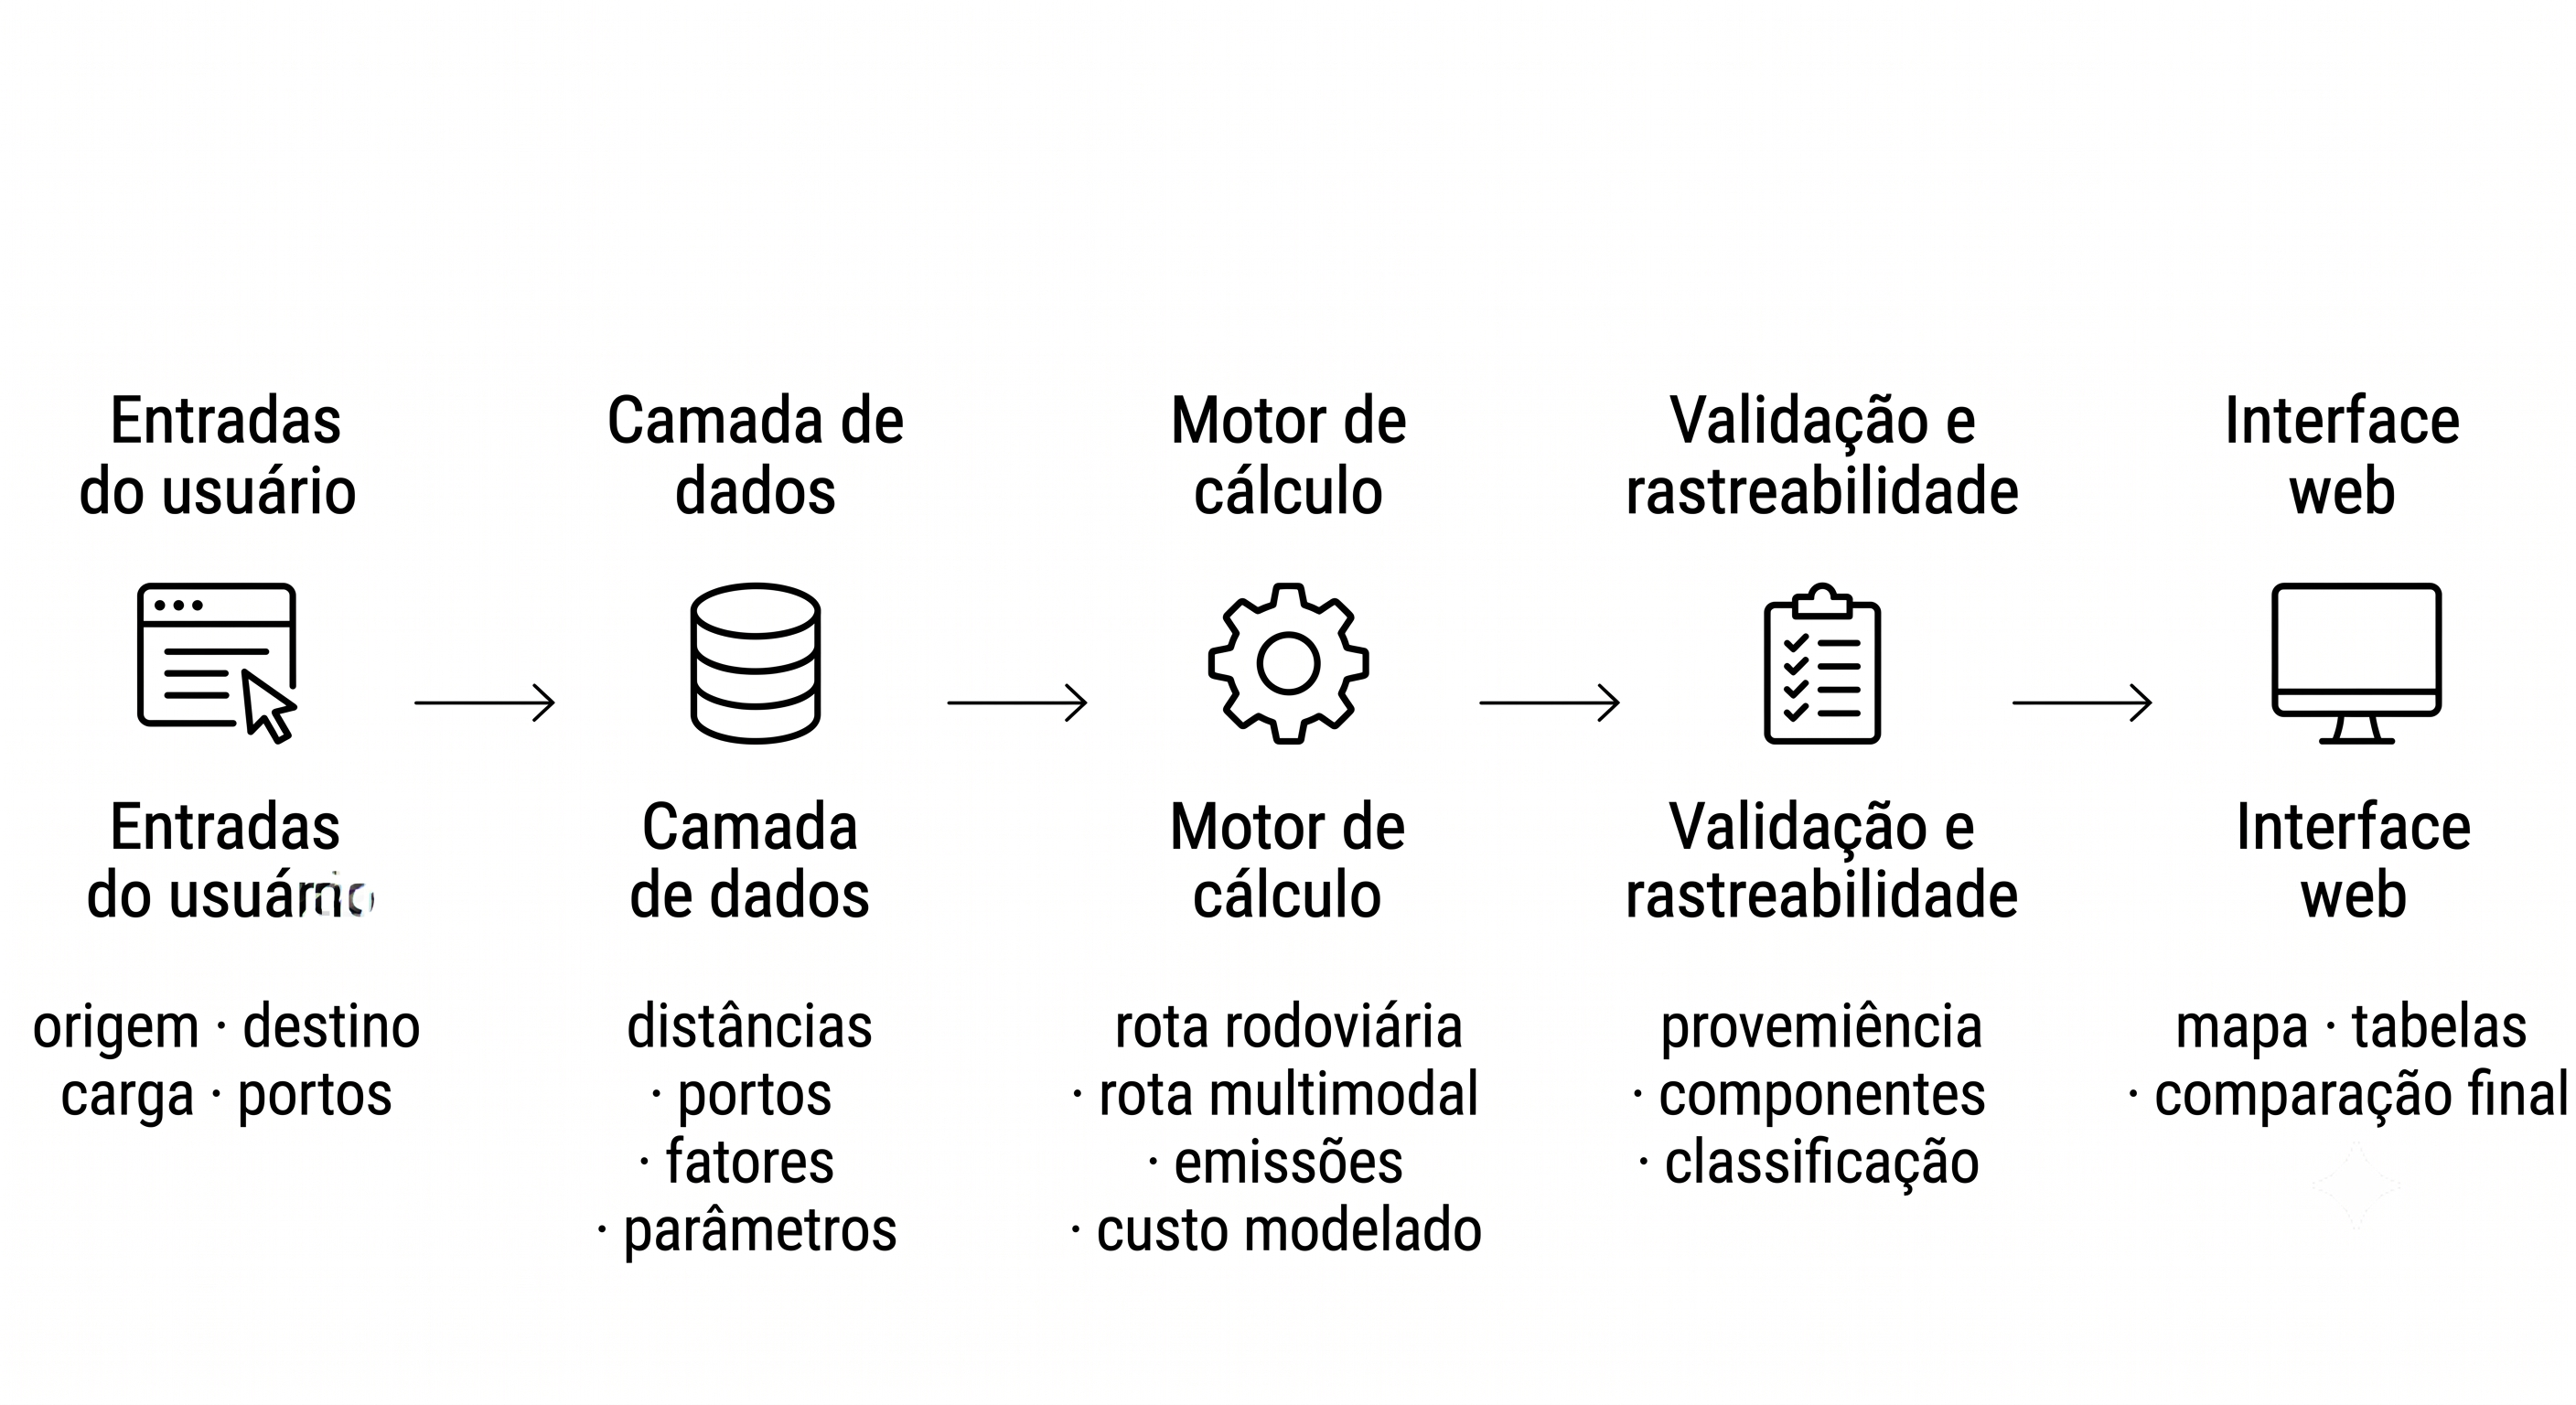
\includegraphics[width=0.95\textwidth]{images/figura_5_1.png}
\caption{Arquitetura computacional simplificada da ferramenta, desde as entradas do usuário e a camada de dados até o motor de cálculo, a rastreabilidade e a interface web.}
\label{fig:arquitetura-computacional}
\end{figure}

\section{Dois fluxos computacionais: execução do cenário e preparação histórica}
\label{sec:fluxos-computacionais}

O sistema possui dois fluxos. Eles se complementam, mas não são executados ao mesmo tempo.

O primeiro é a \textbf{execução de cenário}. Ele começa quando o usuário informa a origem da carga, o destino final da carga e a massa da remessa. A sequência é: entrada do cenário \(\rightarrow\) localização dos pontos no mapa \(\rightarrow\) cálculo ou reaproveitamento das rotas terrestres \(\rightarrow\) seleção do porto de embarque e do porto de desembarque \(\rightarrow\) consulta da matriz marítima já preparada \(\rightarrow\) obtenção dos dados necessários \(\rightarrow\) cálculo de cada parte da viagem \(\rightarrow\) resultados e avisos.

O segundo é a \textbf{preparação dos dados históricos}, realizada antes das simulações do usuário. O processo baixa e integra as tabelas da ANTAQ. Depois, separa os registros por viagem e coloca as escalas da mais antiga para a mais recente. O sistema calcula a carga histórica que permaneceu no navio em cada trecho. Em seguida, procura no EU MRV o consumo correspondente ao IMO. Quando não encontra o IMO, aplica uma regra substituta baseada na classe ou no tipo do navio. Por fim, reúne todas as sequências de portos observadas entre cada porto de embarque e cada porto de desembarque. O resultado é a matriz marítima usada pela aplicação. Quando configurados, Supabase/Postgres ou Supabase Storage podem sincronizar esses arquivos processados.

\begin{table}[htbp]
\centering
\small
\caption{Fluxos computacionais principais do \CabotageLens{}.}
\label{tab:fluxos-computacionais}
\begin{tabularx}{\textwidth}{L{0.22\textwidth}Y Y Y}
\toprule
Fluxo & O que entra & O que transforma & O que entrega ao TF \\
\midrule
Execução de cenário & Origem da carga, destino final da carga, massa da remessa do usuário, portos selecionados e parâmetros. & Consulta rotas e a matriz já preparada; aplica a massa do usuário às distâncias do cenário; calcula combustível, custos e emissões. & Comparação rastreável entre rodovia direta e cadeia multimodal, com avisos e metadados.\\
Preparação histórica offline & Tabelas ANTAQ, dados EU MRV e ativos locais de matriz, preços e parâmetros. & Ordena as escalas da mesma viagem, calcula a carga histórica em cada trecho, busca o consumo por IMO e reúne as diferentes sequências entre portos de embarque e desembarque. & Indicadores marítimos documentados que serão consultados pelos cenários.\\
\bottomrule
\end{tabularx}
\end{table}

A Tabela~\ref{tab:fluxos-computacionais} mostra a separação de responsabilidades. A preparação histórica produz a matriz. A execução consulta essa matriz pronta. A carga histórica a bordo pondera a intensidade durante a preparação. A massa da remessa informada pelo usuário entra somente na execução do cenário. Assim, o sistema não aplica duas vezes a carga histórica.

\section{Entradas do cenário, geocodificação e roteamento terrestre}
\label{sec:entradas-geocodificacao-roteamento}

\textbf{Entradas do usuário.} Um cenário pode conter a origem da carga, o destino final da carga, a massa, o TEU ou a relação t/TEU, a escolha do porto de embarque e do porto de desembarque, a classe de embarcação, o caminhão, o modo de alocação, os preços de combustíveis, as operações portuárias, o \emph{hoteling} e as opções de exportação. A origem e o destino são locais da remessa porta a porta. Os portos delimitam somente a perna marítima.

\textbf{Geocodificação.} O programa transforma nomes de lugares em latitude, longitude, rótulo e UF quando identificável. Primeiro, procura uma coordenada persistida. Se necessário, consulta OpenRouteService. LocationIQ pode atuar como provedor substituto, ou \emph{fallback}, quando configurado. As respostas são normalizadas para que as etapas seguintes não dependam do formato particular de cada provedor.

\textbf{Roteamento terrestre.} Para cada perna rodoviária, o sistema consulta primeiro as rotas já armazenadas no Supabase/Postgres. Somente quando não encontra um registro chama um serviço externo. Essa ordem recebe internamente o nome de \emph{cache-first}. Se o provedor calcular uma rota, o sistema tenta armazenar a resposta.

\textbf{Saída da etapa.} Cada perna terrestre conserva coordenadas, distância, perfil de rota, provedor, fonte e indicação de acerto ou falha de cache. Essas distâncias são rotas modeladas. Elas não são trajetórias GPS observadas nem confirmação de uma rota contratual.

\section{Construção das alternativas, seleção de portos e perna marítima}
\label{sec:construcao-alternativas}

Depois de resolver os lugares, o sistema constrói duas alternativas. A primeira liga a origem da carga ao destino final da carga por rodovia. A segunda divide o percurso em três partes principais: acesso rodoviário da origem da carga ao porto de embarque; navegação até o porto de desembarque; e acesso rodoviário até o destino final da carga. Essa divisão permite medir quanto cada componente contribui para o total.

O porto de embarque e o porto de desembarque podem ser selecionados automaticamente, forçados pelo usuário ou substituídos em uma análise de sensibilidade. A saída identifica qual situação foi usada. A seleção de um porto não confirma frequência, slot, armador ou aceitação terminal.

Para a navegação, o sistema consulta a matriz marítima. A direção importa. Santos--Manaus significa embarcar em Santos e desembarcar em Manaus. Manaus--Santos significa fazer o sentido contrário. A matriz guarda essas duas ligações separadamente. Para cada combinação de porto de embarque e porto de desembarque, ela fornece:

\begin{itemize}
  \item a intensidade representativa calculada com todos os recortes históricos aceitos entre esses portos;
  \item a sequência de portos escolhida para fornecer as distâncias do cenário;
  \item as demais sequências de portos observadas entre a mesma partida e a mesma chegada;
  \item as quantidades de valores obtidos por IMO, classe ou tipo;
  \item a fonte de cada distância marítima.
\end{itemize}

O programa usa uma intensidade para toda a ligação entre o porto de embarque e o porto de desembarque. A intensidade informa quantos gramas de combustível representam o transporte de uma tonelada por uma milha náutica. Para calcular a distância, o programa escolhe uma sequência completa de portos observada. Essa é a rota marítima usada na execução do cenário.

A intensidade calculada somente com os recortes cujo corredor coincide com a sequência escolhida permanece disponível para diagnóstico. Ela não substitui a intensidade representativa calculada com todos os recortes aceitos entre o porto de embarque e o porto de desembarque. Se faltar uma distância positiva entre dois portos diferentes, o sistema pode usar uma aproximação em linha reta baseada nas coordenadas. O identificador interno dessa aproximação é \codecell{haversine\_fallback}. A interface avisa quando isso ocorre. Avisos de mesmo porto nas duas extremidades (\emph{same-port}), distância ausente e regra substituta limitam a interpretação.

\section{Pipeline marítimo offline}
\label{sec:pipeline-maritimo-offline}

O processamento feito antes do uso da aplicação produz a matriz marítima. Ele prepara indicadores históricos; não calcula ainda a remessa do usuário. Internamente, esse processamento recebe o nome de \emph{pipeline offline}. As etapas seguem esta ordem:

\begin{enumerate}
  \item reunir as chamadas do mesmo navio pelo IMO, ordená-las por data e iniciar uma nova viagem quando o navio retorna ao porto inicial ou quando o intervalo entre paradas supera 240 horas;
  \item dentro da mesma viagem, manter as atracações da mais antiga para a mais recente e padronizar os nomes dos portos;
  \item consolidar chamadas consecutivas no mesmo porto sem perder embarques ou desembarques;
  \item reconstruir a carga histórica a bordo com as Equações~\ref{eq:carga-inicial-maritima} e \ref{eq:carga-bordo-subtrecho};
  \item verificar se a viagem realmente percorreu a direção pedida. No cálculo Santos--Manaus, por exemplo, a parte aproveitada da viagem precisa começar na escala de Santos e terminar na escala de Manaus. O sistema usa o recorte Santos--Suape--Pecém--Manaus da viagem real \codecell{voyage\_9612791\_00011}; uma passagem em que Manaus apareça antes de Santos não entra;
  \item conservar todos os trechos consecutivos entre os dois portos, tanto em passagens diretas quanto em passagens com portos intermediários;
  \item manter no máximo um recorte histórico viagem--OD por viagem e por ligação; diante de repetição, preferir a passagem direta e depois a sequência completa de menor distância, o menor número de trechos e a ordem das escalas;
  \item procurar a intensidade pelo IMO, pela classe e pelo tipo, nessa ordem; registrar quando nenhum deles fornecer um valor positivo;
  \item reunir os recortes que receberam uma intensidade, aplicar os pesos de trabalho de transporte e escolher separadamente uma sequência de portos para fornecer as distâncias do cenário.
\end{enumerate}

Para cada recorte aceito, o sistema guarda somente o deslocamento entre os dois portos escolhidos. Esse objeto recebe o nome de \emph{recorte histórico viagem--OD}, em que OD significa origem--destino. Ele contém todos os subtrechos consecutivos entre o porto inicial e o porto final. Cada subtrecho armazena os portos inicial e final, sua posição na sequência, a carga em toneladas e TEU, a distância, a fonte da distância, o trabalho de transporte, a intensidade, o combustível e a indicação de que nenhum subtrecho está ausente. A mesma estrutura representa recortes diretos e recortes com escalas.

A carga histórica muda depois de cada escala. O sistema soma o que foi embarcado e subtrai o que foi desembarcado. Na viagem \codecell{voyage\_9612791\_00011}, a carga inicial reconstruída foi \(2.976{,}894\)~t. O saldo de \(+9.881{,}860\)~t em Santos fez o navio seguir para Suape com \(12.858{,}754\)~t. Depois do saldo de \(+3.859{,}579\)~t em Suape, ele seguiu para Pecém com \(16.718{,}333\)~t. O saldo de \(-4.392{,}433\)~t em Pecém reduziu a carga do trecho seguinte, até Manaus, para \(12.325{,}900\)~t. Essa reconstrução define o peso histórico do indicador. Ela não substitui a massa da remessa informada pelo usuário durante a execução.

O sistema procura primeiro a intensidade do próprio navio pelo IMO. A intensidade mede gramas de combustível por tonelada-milha náutica. Para o IMO, o sistema utiliza o valor positivo mais recente do MRV. Esse valor individual não é alterado pela regra de retirada de valores extremos.

Se o IMO não tiver correspondência, o sistema segue regras substitutas definidas antes do cálculo. Essas regras recebem o nome de fallback.

\textbf{Fallback por classe.} Quando conhece a classe do navio, o sistema usa primeiro a média registrada no arquivo de eficiência depois de excluir os valores abaixo do percentil 1 e acima do percentil 99. Se essa média não estiver disponível, usa a mediana da classe.

\textbf{Fallback por tipo.} Se a classe não fornecer um valor positivo, o sistema reúne os valores positivos mais recentes dos navios do mesmo tipo. Ordena os valores, remove \(\lfloor0{,}01n\rfloor\) de cada extremidade e calcula a média do restante. Se a amostra for pequena demais para remover pelo menos um valor de cada lado, usa a mediana do tipo. Para carga conteinerizada, pode usar o tipo-padrão documentado \emph{Container ship}.

Se IMO, classe e tipo não fornecerem uma intensidade positiva, o sistema registra que o valor não está disponível. Ele não troca a ausência por zero.

O sistema reúne todos os recortes aprovados para a direção pedida. No cálculo Santos--Manaus, por exemplo, entram tanto o recorte direto da viagem \codecell{voyage\_9612789\_00004} quanto o recorte Santos--Suape--Pecém--Manaus da viagem \codecell{voyage\_9612791\_00011}. Uma passagem Manaus--Santos não entra, pois representa a direção contrária. Em cada recorte aprovado, o sistema multiplica a carga a bordo pela distância de cada trecho e soma os produtos. Essa soma é o trabalho de transporte.

O trabalho de transporte funciona como peso na Equação~\ref{eq:mediana-ponderada-intensidade}. O sistema ordena as intensidades e escolhe a primeira que alcança pelo menos metade do peso total acumulado. Esse resultado é a mediana ponderada. Pesos nulos são ignorados quando existe trabalho positivo. Se todos forem nulos, o sistema usa a mediana sem pesos e registra essa condição.

Depois, o sistema escolhe uma única sequência de portos para fornecer as distâncias do cenário. A regra procura primeiro uma ligação direta. Se ela não existir, escolhe a sequência completa de menor distância. O identificador interno dessa regra é \codecell{direct\_first\_then\_shortest\_distance\_km}. Essa escolha define apenas o caminho. Ela não retira nenhum dos demais recortes usados na mediana ponderada.

O sistema gera um arquivo com formato obrigatório, identificado como versão 3. Nesse arquivo ficam registrados a intensidade, sua fonte, o método aplicado, os pesos, a quantidade de viagens, o trabalho total, o uso de valores por IMO ou de estimativas por classe e tipo, a sequência de portos escolhida, os trechos alternativos, a regra usada para reconstruir a carga, o tratamento de valores extremos, a data de geração e os arquivos consultados. O sistema rejeita uma ligação quando falta alguma informação obrigatória ou quando nenhuma distância positiva pode ser usada.

Para auditar uma viagem específica sem produzir milhares de linhas, o pipeline aceita o identificador da viagem e o modo de log detalhado. Por exemplo, a combinação \codecell{--audit-voyage-id voyage\_9612791\_00011} com \codecell{--log-level DEBUG} mostra, para cada subtrecho, o saldo de carga na escala de partida, a carga inicial reconstruída, a carga a bordo, a distância em quilômetros e milhas náuticas, a fonte da distância, o trabalho de transporte, a intensidade, sua fonte e o combustível calculado. O mesmo diagnóstico registra qual viagem cruza o ponto de 50\% da mediana ponderada. Esses logs apenas expõem valores intermediários; não alteram as fórmulas nem o arquivo resultante.

\section{Operacionalização computacional dos insumos metodológicos}
\label{sec:operacionalizacao-insumos}

Os insumos descritos na Seção~\ref{sec:fontes-dados} são usados por componentes com responsabilidades específicas. Cada componente recebe uma entrada, executa uma transformação e devolve uma saída com metadados.

No fluxo online, o programa tenta reaproveitar resultados persistidos antes de chamar provedores. No fluxo offline, scripts atualizam e enriquecem os dados. Em ambos, são registrados o provedor, o cache, a fonte, a regra substituta (\emph{fallback}), o componente incluído ou excluído e os avisos.

\begin{table}[htbp]
\centering
\footnotesize
\setlength{\tabcolsep}{3pt}
\renewcommand{\arraystretch}{1.15}
\caption{Componentes computacionais e metadados preservados.}
\label{tab:componentes-computacionais}
\begin{tabularx}{\textwidth}{L{0.22\textwidth}L{0.23\textwidth}Y Y}
\toprule
Componente computacional & Insumo metodológico usado & Transformação realizada pelo software & Metadado preservado \\
\midrule
Fachada de geocodificação e roteamento & OpenRouteService e LocationIQ como provedores de rota/localização. & Resolve coordenadas, normaliza respostas de provedor e constrói pernas rodoviárias quando não há reaproveitamento persistido. & Provedor, status de cache, perfil de rota, coordenadas, metadados retornados, falhas e provedores substitutos (\emph{fallbacks}).\\
Construtor de pernas rodoviárias & Distâncias terrestres modeladas, origem e destino da carga resolvidos e configuração do cenário. & Procura primeiro uma rota armazenada e, se necessário, chama o provedor; internamente, \emph{cache-first} e \emph{provider-second}. & Chave de consulta, resultado encontrado ou não no cache (\emph{hit/miss}), distância, fonte computacional e avisos de rota modelada.\\
Construtor da perna marítima & Matriz marítima no formato obrigatório versão 3 (\emph{schema 3}), estatísticas ANTAQ/EU MRV e fontes registradas para cada ligação e sequência de portos. & Obtém o consumo representativo, escolhe uma sequência direta ou com paradas e sinaliza aproximação em linha reta (\codecell{haversine\_fallback}) quando necessário. & Método, escopo, peso, fontes IMO/classe/tipo, sequência selecionada, alternativas, trechos e fontes de distância.\\
Resolvedor de insumos de custo & CSV processado de diesel por UF e entrada de bunker/Santos VLSFO associada a Ship \& Bunker. & Prepara os preços usados na estimativa de custo dos trechos rodoviários e marítimos. & UF consultada, fonte do preço, uso de valor-padrão ou substituto, data quando disponível e itens incluídos no custo modelado.\\
Avaliador por trecho & Configurações de caminhão, consumo por tonelada-milha náutica, caminho marítimo, operações portuárias e \emph{hoteling}. & Calcula combustível, estimativa parcial de custo e emissões produzidas durante a operação de cada componente. & Detalhes por trecho, intensidade aplicada, intensidade calculada somente com os recortes da sequência escolhida, fontes IMO ou fallback, componentes incluídos ou excluídos, forma de atribuir o consumo à carga e avisos de dupla contagem.\\
Fluxo offline de atualização & Tabelas ANTAQ, planilhas EU MRV e arquivos locais de matriz e parâmetros. & Calcula a carga em cada trecho, aplica a hierarquia IMO/classe/tipo, trata valores extremos e obtém a mediana ponderada da ligação. & Versões, arquivos processados, política de valores extremos, cobertura, contagens por fonte, ligações e sequências de portos registradas.\\
Camada de persistência e exportação & Rotas, lugares, cenários e resultados computados. & Reutiliza registros, evita chamadas externas repetidas, guarda resultados e produz saídas CSV/JSON quando o fluxo solicita. & Identificador persistido, resultado encontrado ou não no cache (\emph{hit/miss}), registros armazenados, campos exportados e classificação/aviso associado.\\
\bottomrule
\end{tabularx}
\end{table}

Supabase/Postgres e Supabase Storage pertencem à infraestrutura. Eles armazenam registros e arquivos processados. Não substituem a ANTAQ, o EU MRV ou as demais fontes primárias. A qualidade continua dependendo do dado original e da transformação documentada.

\section{Cálculo de cada trecho: combustível, custo operacional estimado e emissões}
\label{sec:calculo-por-perna}

O avaliador calcula uma perna de cada vez. Para a rodovia, recebe distância, carga, caminhão, diesel e fatores implementados. Para a navegação, recebe a intensidade da ligação entre o porto de embarque e o porto de desembarque. Também recebe a massa e as distâncias marítimas. Depois, converte o combustível em custo modelado e emissões operacionais.

Na perna marítima, o cálculo de cada trecho é \(I_{o,d}m_{\mathrm{cen}}d_s/1000\). Nessa expressão, a intensidade \(I_{o,d}\) informa os gramas de combustível por tonelada-milha náutica. A massa \(m_{\mathrm{cen}}\) é a carga informada pelo usuário. A distância \(d_s\) pertence ao trecho calculado. A soma de todos os trechos fornece o combustível de navegação em quilogramas.

O sistema também mostra, para diagnóstico, o valor calculado somente com os recortes cujo corredor coincide com a sequência de portos escolhida. No entanto, o cálculo principal usa a intensidade representativa de todos os recortes aceitos entre os dois portos. A Seção~\ref{sec:intensidade-maritima} explica essa diferença.

\methodnote{\textbf{Exemplo somente da perna marítima Santos--Manaus dentro do cenário São Paulo--Manaus, com 14~t.} \textbf{Entrada do usuário:} origem da carga em São Paulo, destino final da carga em Manaus e massa da remessa de 14~t. \textbf{Portos da navegação:} embarque em Santos e desembarque em Manaus. \textbf{Consulta da matriz histórica:} a intensidade preparada para a ligação Santos--Manaus é \(9{,}322050~\mathrm{g/(t\,nm)}\). A distância selecionada é \(3\,300{,}216~\mathrm{nm}\). \textbf{Cálculo da navegação:} \(9{,}322050\times14\times3\,300{,}216/1000 = 430{,}7069~\mathrm{kg}\). \textbf{Saída arredondada da perna marítima:} 430,71~kg de combustível de navegação. Esse número não é o consumo porta a porta. O acesso rodoviário São Paulo--Santos, o acesso final em Manaus e as operações portuárias são calculados separadamente. Só depois esses componentes entram no total multimodal.}

Esse exemplo também esclarece a diferença entre os dois momentos. Na preparação histórica offline, as cargas a bordo das viagens ANTAQ e os valores MRV produziram a intensidade \(9{,}322050~\mathrm{g/(t\,nm)}\). Na execução, o sistema não reconstrói novamente essas viagens e não soma novamente suas cargas. Ele consulta a intensidade pronta, aplica somente as 14~t informadas pelo usuário e percorre a distância selecionada.

Se o arquivo obrigatório de versão 3 não contiver todos os campos exigidos ou nenhuma distância positiva puder ser usada, o sistema rejeita a ligação e informa que o resultado está indisponível. Ele não transforma a ausência em zero nem apresenta um valor sem identificar sua fonte.

Os componentes de operações portuárias e \emph{hoteling} são calculados conforme a fronteira do cenário. O sistema informa se o dado veio de uma medição específica da operação naquele porto, de uma média entre portos, de um padrão documentado ou se está indisponível. Esse registro da fonte e do tratamento é a proveniência. Quando a intensidade MRV por trabalho de transporte é aplicada, o \emph{hoteling} separado é omitido para evitar dupla contagem. Se um modo o calcula separadamente, horas, chamadas, fonte e fronteira ficam registradas.

Por fim, o sistema soma os componentes. A alternativa rodoviária contém um único trecho. A alternativa multimodal contém o acesso rodoviário inicial, a navegação, as atividades portuárias incluídas e o acesso rodoviário final. O valor econômico continua sendo uma estimativa parcial de custo operacional. Ele não é frete, tarifa, contrato ou preço de mercado.

\section{Persistência, cache, interface e rastreabilidade}
\label{sec:persistencia-cache-interface}

Supabase/Postgres funciona como memória operacional. Quando uma coordenada, rota ou resultado equivalente já existe, o programa pode reutilizá-lo. O reaproveitamento de um dado armazenado recebe o nome técnico de \emph{cache hit}. Ele não comprova que o valor está calibrado, que existe serviço marítimo ou que o custo corresponde ao mercado.

A matriz marítima pode vir de um arquivo local rastreado ou de um arquivo sincronizado. O carregador verifica se o arquivo contém as sequências de portos observadas, a estrutura obrigatória, a data e todos os campos necessários. Havendo mais de um arquivo, seleciona o arquivo completo e mais recente no formato versão 3, identificado internamente como \emph{schema 3}. Um arquivo incompleto não substitui outro que preserve intensidade, método, fonte e contagens.

Na interface Streamlit, os cartões resumem distância, custo modelado e emissões operacionais \ttw{} de \cooe{}. As tabelas mostram cada trecho, os portos, a intensidade, a forma de reunir as viagens, a quantidade de dados obtidos por IMO/classe/tipo, a sequência de portos escolhida, as fontes, os componentes e os avisos. As exportações CSV/JSON preservam entradas, saídas, status, bloqueios, sensibilidades e classificações quando disponíveis.

O código e os arquivos processados rastreados estão no repositório público \url{https://github.com/pennylanesccp/cabotage-lens} \cite{cabotagelensrepo}. A aplicação está publicada em \url{https://cabotagelens.streamlit.app/} \cite{cabotagelensapp}. Esses endereços permitem acessar o protótipo e sua implementação. Eles não substituem as fontes metodológicas.

A principal saída computacional não é apenas um número. É uma trilha auditável: entrada \(\rightarrow\) coordenada \(\rightarrow\) rota \(\rightarrow\) porto \(\rightarrow\) intensidade e distância marítima \(\rightarrow\) combustível \(\rightarrow\) custo e emissões \(\rightarrow\) avisos.

\section{Limitações computacionais e uso correto da ferramenta}
\label{sec:limitacoes-computacionais}

O uso do \CabotageLens{} é analítico e acadêmico. Ele apoia comparação de cenários, sensibilidade, rastreabilidade e identificação de lacunas. Não automatiza contratação, decisão comercial ou validação operacional.

As emissões são operacionais \ttw{} de \cooe{}, salvo indicação diferente. As rotas OpenRouteService/LocationIQ são modeladas, e não GPS observado. A ANTAQ e o EU MRV fortalecem a evidência marítima, mas não provam disponibilidade futura de serviço. Cache e persistência melhoram a reprodução do cálculo, mas não validam preço de mercado ou viabilidade comercial.

Portos alternativos, aproximações em linha reta (\codecell{haversine\_fallback}), avisos de mesmo porto nas duas extremidades (\emph{same-port}) e referências ausentes devem permanecer visíveis. Por isso, a validação do Capítulo~\ref{ch:validacao} interpreta cada saída junto com suas entradas, fontes, componentes e avisos. A ferramenta mostra como o resultado foi produzido; a força da conclusão depende da qualidade da evidência do cenário.
